\section{examples}

\begin{example2}{Multiple Choice} $\surd$ wahr, $\mathrm{x}$ falsch
    \begin{itemize}
        \item $\boxtimes$ Für beliebige Vektoren $\vec{a}, \vec{b}, \vec{c} \in \mathbb{R}^{3}$ gilt $\vec{a} \times \vec{b}=\vec{a} \times \vec{c} \Rightarrow \vec{b}=\vec{c}$
        \item $\surd$ Eine Rotationsmatrix $R=\left(\begin{array}{cc}\cos \varphi & -\sin \varphi \\ \sin \varphi & \cos \varphi\end{array}\right)$ ist immer invertierbar.
        \item $\boxtimes$ Wenn sich der Nullvektor $\overrightarrow{0}$ als Linearkombination $\lambda_{1} \overrightarrow{v_{1}}+\lambda_{2} \overrightarrow{v_{2}}+\cdots+\lambda_{n} \overrightarrow{v_{n}}$ darstellen lässt, sind $\overrightarrow{v_{1}}, \overrightarrow{v_{2}}, \ldots, \overrightarrow{v_{n}}$ linear abhängig.
        \item $\surd$ Sei $\mathbb{V}$ ein Vektorraum. Ist $\operatorname{dim}(\mathbb{V})=0$, dann muss $\mathbb{V}$ der Nullvektorraum (nur der Nullvektor) sein.
        \item $\surd$ Nur Geraden in der Ebene können durch eine Koordinatendarstellung beschrieben werden
        \item $\mathrm{x}$ Die orthogonale Projektion ist invertierbar
    \end{itemize}

    
\end{example2}

\begin{example2}{LGS Lösungsmenge}
    Gegeben ist die erweiterte Koeffizientenmatrix eines linearen Gleichungssystems durch

    $$
    \left(\begin{array}{ccc|c}
    1 & 2 & a+1 & 1 \\
    0 & 3 a & -5 & 20 \\
    0 & 0 & a-1 & 4
    \end{array}\right)
    $$

    Dabei ist $a \in \mathbb{R}$ ein Parameterwert.

    \begin{itemize}
        \item Für welchen Wert von $a$ hat das LGS keine Lösung?
        \item Für welchen Wert von $a$ hat das LGS genau eine Lösung?
        \item Für welchen Wert von $a$ hat das LGS unendlich viele Lösungen?
    \end{itemize}

    \textbf{Lösung:}

    Falls $a=1$ : keine Lösung , da $\left(\begin{array}{ccc|c}1 & 2 & 2 & 1 \\ 0 & 3 & -5 & 20 \\ 0 & 0 & 0 & 4\end{array}\right)$

    Falls $a \neq 1$ und $a \neq 0$ : genau eine Lösung

    Falls $a=0$ : unendlich viele Lösungen, da

    $$
    \left(\begin{array}{ccc|c}
    1 & 2 & 1 & 1 \\
    0 & 0 & -5 & 20 \\
    0 & 0 & -1 & 4
    \end{array}\right) \sim\left(\begin{array}{ccc|c}
    1 & 2 & 1 & 1 \\
    0 & 0 & 1 & -4 \\
    0 & 0 & 0 & 0
    \end{array}\right)
    $$

    Lösungsmenge:

    $\left(\begin{array}{ccc|c}1 & 2 & 1 & 1 \\ 0 & 0 & 1 & -4 \\ 0 & 0 & 0 & 0\end{array}\right)$ erhalten wir: $x_{3}=-4 ; x_{2}=\lambda ; x_{1}=5-2 \lambda$

    bzw.: $\vec{x}=\left(\begin{array}{c}5 \\ 0 \\ -4\end{array}\right)+\lambda\left(\begin{array}{c}-2 \\ 1 \\ 0\end{array}\right)$ mit $\lambda \in \mathbb{R}$

\end{example2}

\columnbreak

\begin{example2}[breakable]{Vektorgeometrie}

    Von einem Parallelogramm $A B C D$ sind die Ecken ist $A=(-1 ;-6 ; 5)$ und $B=(1 ;-1 ; 11)$ gegeben. Die Gerade $g: \vec{r}=\begin{psmallmatrix}11 \\ -6 \\ 8\end{psmallmatrix}+t\begin{psmallmatrix}-2 \\ 2 \\ -1\end{psmallmatrix}$ steht senkrecht auf der Ebene des Parallelogramms und verläuft durch die Ecke $C$.

    \begin{center}
        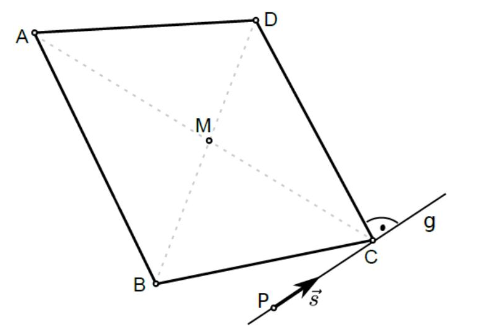
\includegraphics[width=0.6\textwidth]{bsp_vektorgeometrie.png}
    \end{center}

    Bestimmen Sie den Abstand des Ursprungs $O=(0 ; 0 ; 0)$ von der Geraden $g$:

    \resizebox{\columnwidth}{!}{
    mit $F=|\vec{a} \times \overrightarrow{O P}|=\left|\begin{psmallmatrix}-2 \\ 2 \\ -1\end{psmallmatrix} \times\begin{psmallmatrix}11 \\ -6 \\ 8\end{psmallmatrix}\right|=\left|\begin{psmallmatrix}10 \\ 5 \\ -10\end{psmallmatrix}\right|=\left|5 \cdot\begin{psmallmatrix}2 \\ 1 \\ -2\end{psmallmatrix}\right|=15$
    }

    und $|\vec{a}|=\left|\begin{psmallmatrix}-2 \\ 2 \\ -1\end{psmallmatrix}\right|=3$
    ergibt sich: $l=\frac{F}{|\vec{a}|}=\frac{15}{3}=5$

    \vspace{3mm}

    Bestimmen Sie die Koordinatengleichung der Ebene, in der das Parallelogramm liegt:

    Normalenvektor: $\vec{n}=\begin{psmallmatrix}-2 \\ 2 \\ -1\end{psmallmatrix}$ und einem der beiden Punkte $A$ oder $B$ in der Ebene liefert: $d=-\vec{n} \cdot \vec{r}(A)=-\begin{psmallmatrix}-2 \\ 2 \\ -1\end{psmallmatrix} \cdot\begin{psmallmatrix}-1 \\ -6 \\ 5\end{psmallmatrix}=-(2-12-5)=15$ $E:-2 x_{1}+2 x_{2}-x_{3}+15=0$

    \vspace{3mm}

    Berechnen Sie den spitzen Winkel zwischen den Diagonalen des Parallelogramms:

    $\varphi=\arccos \left(\frac{\overrightarrow{A C} \cdot \overrightarrow{B D}}{|\overrightarrow{A C}| \cdot|\overrightarrow{B D}|}\right)$ mit $\overrightarrow{A C}=\begin{psmallmatrix}5+1 \\ 0+6 \\ 5-5\end{psmallmatrix}=\begin{psmallmatrix}6 \\ 6 \\ 0\end{psmallmatrix}$ 
    
    und $\overrightarrow{B D}=\begin{psmallmatrix}3-1 \\ -5+1 \\ -1-11\end{psmallmatrix}=\begin{psmallmatrix}2 \\ -4 \\ -12\end{psmallmatrix}$

    $
    \begin{aligned}
    \varphi & =\arccos \left(\frac{\overrightarrow{A C} \cdot \overrightarrow{B D}}{|\overrightarrow{A C}| \cdot|\overrightarrow{B D}|}\right)=\arccos \left(\frac{\begin{psmallmatrix}6 \\ 6 \\ 0\end{psmallmatrix} \cdot\begin{psmallmatrix}2 \\ -4 \\ -12\end{psmallmatrix}}{6 \sqrt{2} \cdot 2 \sqrt{41}}\right)\\ 
    & =\arccos \left(-\frac{12}{12 \sqrt{82}}\right) =\arccos \left(-\frac{1}{\sqrt{82}}\right) \approx 83.66^{\circ}
    \end{aligned}
    $

    \vspace{3mm}

    Bestimmen Sie die Koordinaten der Ecke $C$:

    Schnittpunkt von $E$ und $g$ ( $g$ in $E$,,einsetzen“)

    aus $g: \vec{r}=\begin{psmallmatrix}11 \\ -6 \\ 8\end{psmallmatrix}+t\begin{psmallmatrix}-2 \\ 2 \\ -1\end{psmallmatrix}$ 
    
    ergibt sich $x_{1}=11-2 t ; x_{2}=-6+2 t ; x_{3}=8-t$

    eingesetzt in $\quad E:-2 x_{1}+2 x_{2}-x_{3}+15=0$
    ergibt sich: 
    
    $-2(11-2 \lambda)+2(-6+2 \lambda)-(8-\lambda)+15=0$

    $
    -22+4 \lambda-12+4 \lambda-8+\lambda+15=0
    \Rightarrow
    -27+9 \lambda=0 \Rightarrow \lambda=3
    $

    eingesetzt in $g$ ergibt sich $C=(5 ; 0 ; 5)$

    \vspace{6mm}

    Bestimmen Sie die Koordinaten der Ecke $D$:

    Das kann man nun über die Information lösen, dass es sich um ein Parallelogramm handelt:

$
\vec{r}(D)=\vec{r}(C)+\overrightarrow{B A}=\left(\begin{array}{l}
5 \\
0 \\
5
\end{array}\right)+\left(\begin{array}{l}
-1-1 \\
-6+1 \\
5-11
\end{array}\right)=\left(\begin{array}{l}
5 \\
0 \\
5
\end{array}\right)+\left(\begin{array}{l}
-2 \\
-5 \\
-6
\end{array}\right)=\left(\begin{array}{c}
3 \\
-5 \\
-1
\end{array}\right)
$

\end{example2}



\begin{example2}{Spezialfall Matrixmultiplikation} $AB = BA$ für $2\times 2$ Matrizen
    
        Seien $A=\left(\begin{array}{cc}a & b \\ c & d\end{array}\right)$ und $B=\left(\begin{array}{cc}1 & 2 \\ 2 & 3\end{array}\right)$ zwei $2 \times 2$-Matrizen. Dann gilt:
    
        Es gilt $AB = BA$ genau dann, wenn $A = \begin{psmallmatrix}
            \lambda-\mu & mu \\ \mu & \lambda
        \end{psmallmatrix}$
\end{example2}

\begin{example2}{Determinante} mit Laplace-Entwicklung
    $A^{4 \times 4} = \begin{psmallmatrix}
        1 & 1 & 0 & 0 \\
        0 & 1 & 0 & -1 \\
        0 & 0 & 1 & -1 \\
        2 & 0 & 0 & 1
    \end{psmallmatrix}$

    Entwickeln Sie die Determinante von $A$ nach der 3. Spalte

    $
    \begin{aligned}
    \operatorname{det}(A) & =1 \cdot(-1)^{3+3} \cdot \operatorname{det}\left(\begin{array}{ccc}1 & 1 & 0 \\ 0 & 1 & 0 \\ 2 & 0 & 1\end{array}\right) \\
    & =1 \cdot(-1) \cdot\left(1 \cdot(-1)^{3+3} \cdot \operatorname{det}\left(\begin{array}{cc}1 & 0 \\ 0 & 1\end{array}\right)+0+0\right) \\
    & =-1 \cdot\left(1 \cdot 1 \cdot(1 \cdot 1-0 \cdot 0)+0+0\right) \\
    & =-1 \cdot(1 \cdot 1)=1
    \end{aligned}
    $
\end{example2}

\begin{example2}{Basis}

    Zeigen Sie, dass $\mathcal{B}=\left\{\begin{psmallmatrix}1 \\ 0 \\ 0\end{psmallmatrix},\begin{psmallmatrix}-3 \\ 1 \\ 0\end{psmallmatrix},\begin{psmallmatrix}4 \\ -2 \\ 1\end{psmallmatrix}\right\}$ eine Basis von $\mathbb{R}^{3}$ ist.
    
    z.B. $\left|\begin{psmallmatrix}1 & -3 & 4 \\ 0 & 1 & -5 \\ 0 & 0 & 1\end{psmallmatrix}\right|=1 \neq 0 \quad \Rightarrow \quad \mathcal{B}$ ist eine Basis von $\mathbb{R}^{3}$

    \vspace{3mm}

    Bestimmen Sie für $\vec{a}=\begin{psmallmatrix}1 \\ -2 \\ 3\end{psmallmatrix}_{\mathcal{S}}$ die Komponentendarstellung bezüglich $\mathcal{B}$.

    Wir müssen das folgende LGS lösen: $\begin{psmallmatrix}1 & -3 & 4 \\ 0 & 1 & -2 \\ 0 & 0 & 1\end{psmallmatrix} \cdot\begin{psmallmatrix}a_{1 b} \\ a_{2 b} \\ a_{3 b}\end{psmallmatrix}=\begin{psmallmatrix}1 \\ -2 \\ 3\end{psmallmatrix}$

    $$
    \begin{psmallmatrix}1 & -3 & 4 & 1 \\ 0 & 1 & -2 & -2 \\ 0 & 0 & 1 & 3\end{psmallmatrix} \leftarrow\left|\cdot 2 \_\right| \cdot(-4) \sim\begin{psmallmatrix}1 & -3 & 0 & -11 \\ 0 & 1 & 0 & 4 \\ 0 & 0 & 1 & 3\end{psmallmatrix} 
    $$
    $$
    \leftarrow  \cdot 3 \sim\begin{psmallmatrix}1 & 0 & 0 & 1 \\ 0 & 1 & 0 & 4 \\ 0 & 0 & 1 & 3\end{psmallmatrix}_{\mathcal{S}}=\begin{psmallmatrix}1 \\ 4 \\ 3\end{psmallmatrix}_{\mathcal{B}}
    $$

    Oder über die Inverse der Matrix:

\resizebox{\columnwidth}{!}{
$
\vec{a}=\left(\begin{array}{ccc}
1 & -3 & 4 \\
0 & 1 & -2 \\
0 & 0 & 1
\end{array}\right)^{-1}\left(\begin{array}{c}
1 \\
-2 \\
3
\end{array}\right)_{\mathcal{S}}=\left(\begin{array}{lll}
1 & 3 & 2 \\
0 & 1 & 2 \\
0 & 0 & 1
\end{array}\right)\left(\begin{array}{c}
1 \\
-2 \\
3
\end{array}\right)_{\mathcal{S}}=\left(\begin{array}{l}
1 \\
4 \\
3
\end{array}\right)_{\mathcal{B}}
$}

    \vspace{3mm}

    Bestimmen Sie für $\vec{b}=\begin{psmallmatrix}3 \\ 2 \\ 1\end{psmallmatrix}_{\mathcal{B}}$ die Komponentendarstellung bezüglich der Standardbasis $\mathcal{S}$.

    Wir müssen nur das Matrizenprodukt berechnen: 
    
    $\vec{b}=\begin{psmallmatrix}3 \\ 2 \\ 1\end{psmallmatrix}_{\mathcal{B}}=\begin{psmallmatrix}1 & -3 & 4 \\ 0 & 1 & -2 \\ 0 & 0 & 1\end{psmallmatrix} \cdot\begin{psmallmatrix}3 \\ 2 \\ 1\end{psmallmatrix}_{\mathcal{B}}=\begin{psmallmatrix}1 \\ 0 \\ 1\end{psmallmatrix}_{S}$

\end{example2}


\begin{example2}[breakable]{Lineare Abbildungen}

    Gegeben sind die folgenden linearen Abbildungen

    $$
    g: \R^5 \rightarrow \R^5, \vec{x} \rightarrow g(\vec{x})=\begin{psmallmatrix}
        x_1 - x_2 + x_4 + x_5 \\
        x_2 + x_3 + 2x_5 \\
        -x_1 + x_2 - 2x_5 \\
        x_4 - x_5 \\
        x_2 + x_3 + 2x_4
    \end{psmallmatrix}
    $$
    $$
    h: \R^5 \rightarrow \R, \vec{x} \rightarrow g(\vec{x})=x_1 + x_2 + x_3 - x_4 - x_5
    $$

Bestimmen Sie jeweils die Darstellungsmatrix der Abbildungen $g$ und $h$.

$$
A_g = \begin{psmallmatrix}
    1 & -1 & 0 & 1 & 1 \\
    0 & 1 & 1 & 0 & 2 \\
    -1 & 1 & 0 & 0 & -2 \\
    0 & 0 & 0 & 1 & -1 \\
    0 & 1 & 1 & 2 & 0
\end{psmallmatrix}
\text{ und }
A_h = \begin{psmallmatrix}
    1 & 1 & 1 & -1 & -1
\end{psmallmatrix}
$$

Bestimmen Sie für die lineare Abbildung $g$ den Kern und das Bild.

Kern bestimmen über Lösen des LGS:

$$
\begin{psmallmatrix}
    1 & -1 & 0 & 1 & 1 & |0 \\
    0 & 1 & 1 & 0 & 2 & |0 \\
    -1 & 1 & 0 & 0 & -2 & |0 \\
    0 & 0 & 0 & 1 & -1 & |0 \\
    0 & 1 & 1 & 2 & 0 & |0
\end{psmallmatrix} \sim 
\begin{psmallmatrix}
    1 & -1 & 0 & 1 & 1 & |0 \\
    0 & 1 & 1 & 0 & 2 & |0 \\
    0 & 0 & 0 & 1 & -1 & |0 \\
    0 & 0 & 0 & 1 & -1 & |0 \\
    0 & 1 & 1 & 2 & 0 & |0
\end{psmallmatrix} 
$$
$$
\sim
\begin{psmallmatrix}
    1 & -1 & 0 & 1 & 1 & |0 \\
    0 & 1 & 1 & 0 & 2 & |0 \\
    0 & 1 & 1 & 2 & 0 & |0 \\
    0 & 0 & 0 & 1 & -1 & |0 \\
    0 & 0 & 0 & 0 & 0 & |0
\end{psmallmatrix} \sim
\begin{psmallmatrix}
    1 & -1 & 0 & 1 & 1 & |0 \\
    0 & 1 & 1 & 0 & 2 & |0 \\
    0 & 0 & 0 & -2 & 2 & |0 \\
    0 & 0 & 0 & 1 & -1 & |0 \\
    0 & 0 & 0 & 0 & 0 & |0
\end{psmallmatrix} \sim
\begin{psmallmatrix}
    1 & -1 & 0 & 1 & 1 & |0 \\
    0 & 1 & 1 & 0 & 2 & |0 \\
    0 & 0 & 0 & 1 & -1 & |0 \\
    0 & 0 & 0 & 0 & 0 & |0 \\
    0 & 0 & 0 & 0 & 0 & |0
\end{psmallmatrix}
$$

mit der Lösung

$$
\operatorname{ker}(A_g) = \left\{\lambda_1\begin{psmallmatrix}-4 \\ -2 \\ 0 \\ 1 \\ 1\end{psmallmatrix} + \lambda_2\begin{psmallmatrix}-1 \\ -1 \\ 1 \\ 0 \\ 0\end{psmallmatrix} \middle| \lambda_1, \lambda_2 \in \mathbb{R}\right\}
$$
Bild: es gilt: $\operatorname{dim}\left(\operatorname{im}\left(A_{g}\right)\right)=\operatorname{dim}\left(\mathbb{R}^{5}\right)-\operatorname{dim}\left(\operatorname{ker}\left(A_{g}\right)\right)=3$
$$
\operatorname{im}\left(A_{g}\right)=\left\{\lambda_{3}\begin{psmallmatrix}1 \\ 0 \\ -1 \\ 0 \\ 0\end{psmallmatrix}+\lambda_{4}\begin{psmallmatrix}0 \\ 1 \\ 0 \\ 0 \\ 1\end{psmallmatrix}+\lambda_{5}\begin{psmallmatrix}1 \\ 0 \\ 0 \\ 1 \\ 2\end{psmallmatrix} \middle| \lambda_{3}, \lambda_{4}, \lambda_{5} \in \mathbb{R}\right\}
$$

Ist die lineare Abbildung $g$ bijektiv? Begründen Sie Ihre Antwort kurz.

Nein. Wir erkennen dies daran, dass die Dimension des Kerns grösser als 0 ist, d.h. es wird also nicht nur der Nullvektor, sondern unendlich viele Vektoren auf den Nullvektor abgebildet.

Damit ist diese Abbildung sicher nicht injektiv (linkseindeutig) und damit nicht bijektiv.

\vspace{3mm}

Geben Sie die Abbildungsmatrix der Abbildung $h \circ g$ an.

Für die Verknüpfung der Abbildungsmatrix der Abbildung $h \circ g$ müssen wir zunächst $g$ dann $h$ ausführen, daher steht die Matrix $A_{g}$ rechts im Matrizenprodukt:

$$
A_h \cdot A_g = \begin{psmallmatrix}
    1 & 1 & 1 & -1 & -1
\end{psmallmatrix} \cdot \begin{psmallmatrix}
    1 & -1 & 0 & 1 & 1 \\
    0 & 1 & 1 & 0 & 2 \\
    -1 & 1 & 0 & 0 & -2 \\
    0 & 0 & 0 & 1 & -1 \\
    0 & 1 & 1 & 2 & 0
\end{psmallmatrix} = \begin{psmallmatrix}
    0 & 0 & 0 & -2
\end{psmallmatrix}
$$

\end{example2}

\begin{example2}{Geometrische Transformationen}
    Der Punkt $P(2|3| 4)$ wird zunächst um $90^{\circ}$ in der gezeichneten Richtung um die $y$-Achse in den Punkt $P^{*}$ gedreht und dieser anschliessend an der $x$-Achse in den Punkt $P^{* *}$ gespiegelt.
    
    \begin{minipage}{0.5\linewidth}
        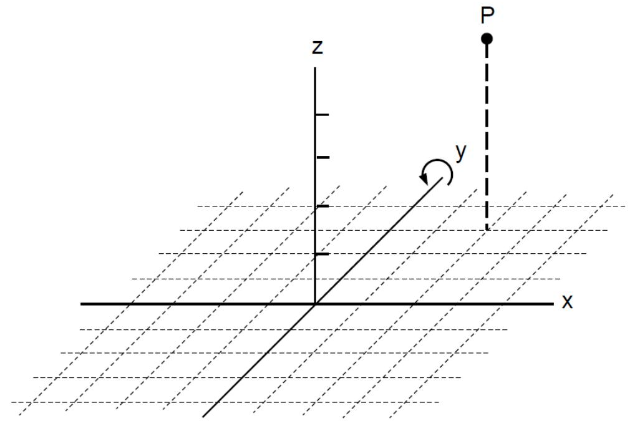
\includegraphics[width=1\linewidth]{geometrie_bsp1.png}
    \end{minipage}
    \begin{minipage}{0.5\linewidth}
        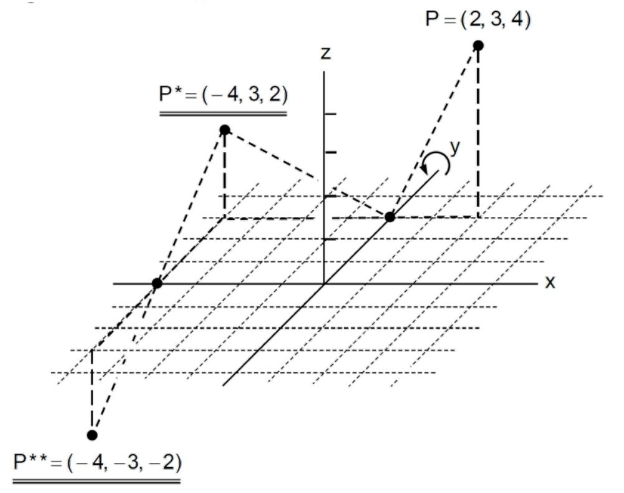
\includegraphics[width=1\linewidth]{geometrie_bsp2.png}
    \end{minipage}

    Bestimmen Sie die Koordinaten des Punktes $P^{*}$ und $P^{* *}$. (siehe Darstellung rechts)

    \vspace{3mm}

    Bestimmen Sie die Matrix $A$ der Drehung, welche $P$ in $P^{*}$ überführt, sowie die Matrix $B$ der Spiegelung, welche $P^{*}$ in $P^{* *}$ überführt.
    
    Die Gesamtabbildung, welche $P^{*}$ in $P^{* *}$ überführt, besitzt die Matrix

    $$
    C=\begin{psmallmatrix}
        0 & 0 & -1 \\
        0 & -1 & 0 \\
        -1 & 0 & 0
    \end{psmallmatrix}
    $$

    Für die Drehung gilt:

    $
    \begin{psmallmatrix}
        1 & 0 & 0
    \end{psmallmatrix} \rightarrow \begin{psmallmatrix}
        0 & 0 & 1
    \end{psmallmatrix} ; \begin{psmallmatrix}
        0 & 1 & 0
    \end{psmallmatrix} \rightarrow \begin{psmallmatrix}
        0 & 1 & 0
    \end{psmallmatrix} ; \begin{psmallmatrix}
        0 & 0 & 1
    \end{psmallmatrix} \rightarrow \begin{psmallmatrix}
        -1 & 0 & 0
    \end{psmallmatrix} \\ \Rightarrow A=\begin{psmallmatrix}
        0 & 0 & -1 \\
        0 & 1 & 0 \\
        1 & 0 & 0
    \end{psmallmatrix}
    $

    \vspace{2mm}

Für die Spiegelung gilt:

$
\begin{psmallmatrix}
    1 & 0 & 0
\end{psmallmatrix} \rightarrow \begin{psmallmatrix}
    1 & 0 & 0
\end{psmallmatrix} ; \begin{psmallmatrix}
    0 & 1 & 0
\end{psmallmatrix} \rightarrow \begin{psmallmatrix}
    0 & -1 & 0
\end{psmallmatrix} ; \begin{psmallmatrix}
    0 & 0 & 1
\end{psmallmatrix} \rightarrow \begin{psmallmatrix}
    0 & 0 & -1
\end{psmallmatrix} \\ \Rightarrow B=\begin{psmallmatrix}
    1 & 0 & 0 \\
    0 & -1 & 0 \\
    0 & 0 & -1
\end{psmallmatrix}
$

\vspace{2mm}

Bestimmen Sie alle Punkte $Q=\left(x_{Q} ; y_{Q} ; z_{Q}\right)$, welche unter der Gesamtabbildung auf sich selbst abgebildet werden.

Es muss also gelten:
$$
C \cdot Q=Q \Rightarrow \begin{psmallmatrix}
    0 & 0 & -1 \\
    0 & -1 & 0 \\
    -1 & 0 & 0
\end{psmallmatrix}
\begin{psmallmatrix}
    x_{Q} \\
    y_{Q} \\
    z_{Q}
\end{psmallmatrix}=\begin{psmallmatrix}
    x_{Q} \\
    y_{Q} \\
    z_{Q}
\end{psmallmatrix} \Rightarrow \begin{psmallmatrix}
    -z_{Q} \\
    -y_{Q} \\
    -x_{Q}
\end{psmallmatrix}= \begin{psmallmatrix}
    x_{Q} \\
    y_{Q} \\
    z_{Q}
\end{psmallmatrix} 
$$
$$
\Rightarrow \begin{aligned}
    & x_{Q}=-z_{Q}=\lambda \\
    & y_{Q}=0
\end{aligned} \Rightarrow Q=\left(\lambda ; 0 ; -\lambda\right) \text { mit } \lambda \in \mathbb{R}
$$

Berechnen Sie $C^{2}$.

Die Abbildung zweifach angewendet ergibt:

$$
C^{2}=\begin{psmallmatrix}
    0 & 0 & -1 \\
    0 & -1 & 0 \\
    -1 & 0 & 0
\end{psmallmatrix} \begin{psmallmatrix}
    0 & 0 & -1 \\
    0 & -1 & 0 \\
    -1 & 0 & 0
\end{psmallmatrix} = \begin{psmallmatrix}
    1 & 0 & 0 \\
    0 & 1 & 0 \\
    0 & 0 & 1
\end{psmallmatrix} = E
$$

Geben Sie aufgrund der Ergebnisse von c) und d) an, was für eine geometrische Transformation die Gesamtabbildung ist.

Die Gesamttransformation $C$ ist mutmasslich eine Spiegelung an der Geraden

$$
g: \lambda \cdot \begin{psmallmatrix}
    1 \\
    0 \\
    -1
\end{psmallmatrix} \text { mit } \lambda \in \mathbb{R}
$$

\end{example2}

\begin{example2}{Vektorgeometrie allgemein}

    Parameterdarstellung einer Geraden $g$, die durch die Punkte $P$ und $Q$ verläuft:
    \begin{itemize}
        \item Wähle P als Fixpunkt
        \item $\vec{P Q}$ als Richtungsvektor
    \end{itemize}
    $\Rightarrow g: \vec{r}=\vec{p}+ \lambda \cdot \vec{PQ}$

    \vspace*{3mm}

    Parameterdarstellung einer Ebene $E$, die durch die Punkte $P, Q$ und $R$ verläuft:
    \begin{itemize}
        \item Wähle $P$ als Fixpunkt
        \item $\vec{PQ}$ und $\vec{PR}$ als Richtungsvektoren
        \item $\vec{n}=\vec{PQ} \times \vec{PR}$ als Normalenvektor
    \end{itemize}
    $\Rightarrow E: \vec{r}=\vec{p}+ \lambda \cdot \vec{PQ} + \mu \cdot \vec{PR}$

    \vspace*{3mm}

    Parameterdarstellung einer Ebene $E$, die durch den Punkt $P$ verläuft und orthogonal zur Geraden $g$ ist:
    \begin{itemize}
        \item Wähle $P$ als Fixpunkt
        \item $\vec{n}$ als Normalenvektor
        \item $\vec{r} \cdot \vec{n} = \vec{p} \cdot \vec{n}$
        \item $\vec{n} \cdot \vec{r} = \vec{n} \cdot \vec{p}$
        \item $\vec{n} \cdot (\vec{r} - \vec{p}) = 0$
    \end{itemize}
    $\Rightarrow E: \vec{n} \cdot (\vec{r} - \vec{p}) = 0$

    \vspace{3mm}

    Koordinatendarstellung einer Ebene $E$, auf der die Punkte $P, Q$ und $R$ liegen:
    \begin{itemize}
        \item Wähle $P$ als Fixpunkt
        \item $\vec{PQ}$ und $\vec{PR}$ als Richtungsvektoren
        \item $\vec{n}=\vec{PQ} \times \vec{PR}$ als Normalenvektor
    \end{itemize}
    $\Rightarrow E: n_1 \cdot x + n_2 \cdot y + n_3 \cdot z + d = 0$
    
    Bestimme d indem du den Normalenvektor $\vec{n}$ und den Punkt $Q$ einsetzt.

    \vspace{3mm}
\end{example2}


\begin{example2}{Rotation{,} Spiegelung und Abbildungsmatrix}
    Betrachte die Punkte $P = (2|1)$ und $Q = (-1|2)$ in der Ebene $E$

    \vspace{3mm}

    Bestimmen Sie die Koordinaten des Punktes $P^{*}$, der durch eine Rotation um $90^{\circ}$ um den Ursprung entsteht.

    $$
    P^{*} = \begin{psmallmatrix}
        0 & -1 \\
        1 & 0
    \end{psmallmatrix} \cdot \begin{psmallmatrix}
        2 \\
        1
    \end{psmallmatrix} = \begin{psmallmatrix}
        -1 \\
        2
    \end{psmallmatrix}
    $$
    
    \vspace{3mm}

    An welcher Gerade $ax + by = c$ muss man den Punkt $P$ spiegeln, damit er auf den Punkt $Q$ abgebildet wird?

    Normalenvektor der Spiegelungsebene: $\vec{n} = \vec{PQ} = \begin{psmallmatrix}
        -3 \\
        1
    \end{psmallmatrix}$

    Einheitsvektor: $\vec{e} = \frac{\vec{n}}{|\vec{n}|} = \begin{psmallmatrix}
        -\frac{3}{\sqrt{10}} \\
        \frac{1}{\sqrt{10}}
    \end{psmallmatrix}$

    Spiegelmatrix: $S = E - 2 \cdot \vec{e} \cdot \vec{e}^{T} = \begin{psmallmatrix}
        0.2 & 0.6 \\
        0.6 & 0.8
    \end{psmallmatrix}$ = $S = \begin{psmallmatrix}
        1 - 2a^2 & -2ab \\
        -2ab & 1 - 2b^2
    \end{psmallmatrix}$
\end{example2}

\begin{example2}{even more geometry shit}

    Bestimme die Koordinaten des Punkt $D$, der ein rechtwinklig-gleichschenkliges Dreieck $ABC$ zu einem Quadrat ergänzt (in $\R^3$):
    $$\vec{r}(D) = \vec{r}(A) + \vec{BC}$$
    
\end{example2}